\chapter{Introduction} \label{chap1}

The problem considered in this thesis arises from the Kronig-Penney model, see for example \cite[Chap. 3]{HeeringEP}, which describes an idealised quantum-mechanical system that models a quantum particle behaving as a matter wave moving in one-dimension through an infinite periodic array of rectangular potential barriers, i.e. through a space area in which a potential attains a local maximum. Such an array commonly occurs in models of periodic crystal lattices where the potential is caused by ions in the crystal structure. Those charged molecules create an electromagnetic field around themselves. Hence, any particle moving through such a crystal would be subject to a recurrent electromagnetic potential. Although a solid particle, simplified as a point mass, would be reflected at such a barrier, there is a possibility that the quantum particle, as it behaves like a wave, penetrates the barrier and continues its movement beyond. Assuming the spacing between all ions is equidistant the potential function $V(x)$ in the lattice can be approximated by a rectangular potential like this:

\begin{figure*}[h!] \centering
	  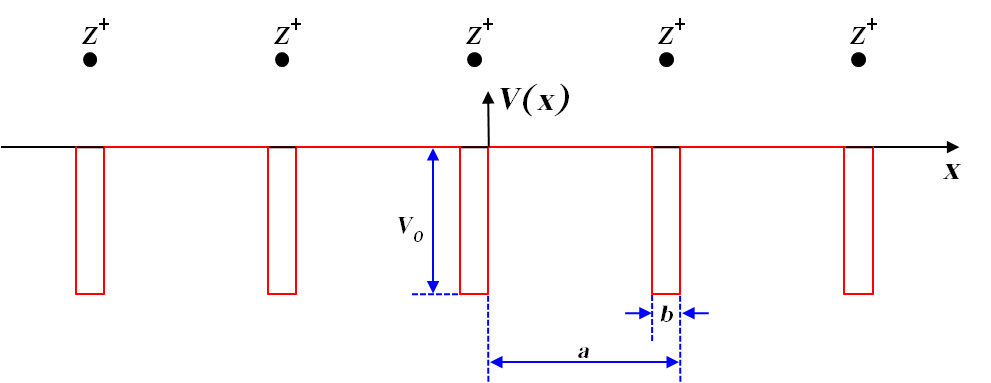
\includegraphics[width=0.75\textwidth]{Periodic_square_potential_130707} 
\end{figure*}

where $b$ is the \enquote{support} and $\rho$ the magnitude of the potential.
~\newpage % temporarily
In this thesis we will examine the spectrum of the operator describing a special case of the Kronig-Penney model, more precisely a model which represents a particle moving through periodically distributed, singular potentials by taking the limit $b \rightarrow 0$ while $V_{0}$ remains in order $\rho b$ in the above described situation.

\section*{Mathematical Basics}

For the upcoming analysis we need some basic concepts from functional analysis and spectral theory I wish to briefly review:
~\newline ~\newline
Let $C_{c}^{\infty}$ denote the linear space containing all smooth function $f \colon \R \rightarrow \R$ with compact support, i.e. for $f \in C_{0}^{\infty}$ there exists a compact interval $I \subseteq \R$ such that $f(x) = 0$ for all $x \notin I$. And will hereafter $\langle x, x \rangle$ denote the scalar product in $L^{2}(\R)$.

\begin{definition}[Weak derivative]
	Let $\Omega \subseteq \R$ be an open set and let $u$ be a function in the Lebesgue space $L^{1}(\Omega)$. Then $v$ in $L^{1}(\Omega)$ is a weak derivative of $u$ if, 
	\[ \int_{\Omega} u(t)\varphi'(t) dt = -\int_{\Omega} v(t) \varphi(t) dt \]
for all $\varphi \in C_{0}^{\infty}(\Omega)$. 
\end{definition}
Now, an important example for a Hilbert space is the Sobolev space $H^{k}(\Omega)$, which is defined to be the set of functions $f$ in $L^{2}(\Omega)$ such that the function $f$ and its weak derivatives up to the order $k$ have a finite $L^{2}(\Omega)$ norm, by admitting the inner product in terms of the $L^{2}(\Omega)$ inner product for all derivatives up to order $k$: 
	\[ \langle u , v \rangle_{H^{k}(\Omega)} = \sum_{i=0}^{k} \left\langle D^{i}u , D^{i} v \right\rangle_{L^{2}(\Omega)}. \] 	

\begin{definition}[Distributions]
	On $C_{0}^{\infty}$ a sequence $(f_{n})$ converges against $f \in C_{0}^{\infty}$ if the support of all members of the sequence is in a compact interval $I \subset \R$, i.e.
	$$ \supp (f_{n}) \subseteq I \quad \forall n \in \N, $$
	and on this interval $f_{n}$ and all its derivatives converge uniformly against $f$, i.e.
	\[ \| f_{n}^{(i)} - f^{(i)} \|_{\infty} \rightarrow 0 \quad \text{ for } n \rightarrow \infty \]
	for all $i \in \N_{0}$. One can proof that this concept of convergence generates a topology on $C_{0}^{\infty}$ and one usually denoted with $\mathcal{D}(\R)$ the space $C_{0}^{\infty}$ equipped with this topology. From now on, we denote with $D'(\R)$ the space of all linear functionals on $C_{0}^{\infty}$ that are continuous with respect to this topology and call those functionals distributions.
\end{definition}
An important example for a distribution is the Dirac delta function $\delta_{x_{0}}$ where $x_{0} \in \R$. It is defined as the limit of a weakly converging sequence of functionals over normed symmetric around $x_{0}$ cumulative distribution functions $\delta_{\epsilon}$, whereas the support of those cumulative distributions converges to zero. It holds $\delta_{x_{0}} = \lim_{\epsilon \rightarrow 0} \delta_{\epsilon}$ in $D'(\R)$. An example for such a sequence is
	\begin{equation}
		\delta_{\epsilon}(x) = \frac{1}{\sqrt{2 \pi} \epsilon} e^{-\frac{x^{2}}{2 \epsilon^{2}}}. \label{smooth-potential}
	\end{equation} 
Which implies the definition
	\[ \delta_{x_{0}}(f) \coloneqq \int_{-\infty}^{\infty} \delta_{x_{0}} f(x) dx \coloneqq \lim_{\epsilon \rightarrow 0} \int_{-\infty}^{\infty} \delta_{\epsilon}(x - x_{0}) f(x) dx. \]
Moreover, is easily seen that $\delta_{x_{0}}(f) = \lim_{\epsilon \rightarrow 0} \delta_{\epsilon}(f) = f(x_{0})$, for a proof see \cite{WeisST}.

\begin{definitions}
Let $X, Y$ be Banach spaces and let $A \colon \mathcal{D}(A) \rightarrow Y$ be a linear operator with domain $\mathcal{D}(A) \supset X$. 
\begin{enumerate}[label=\alph*\upshape)]
	\item We call $A$ closed if $graph(A) \coloneqq \{ (x, Ax) : x \in \mathcal{D}(A) \} \subseteq X \times Y$ is a closed set.
\end{enumerate}
Are $X, Y$ Hilbert spaces and $A$ a bounded operator we call
\begin{enumerate}[label=\alph*\upshape)]  \setcounter{enumi}{1}
	\item $A$ symmetric, if $\langle Tx,y \rangle = \langle x ,Ty \rangle$ for all $x,y \in \mathcal{D}(A)$, and
	\item $A$ self-adjoint, if $A$ is densely defined on $X$ and coincides with its adjoint.
\end{enumerate}
Furthermore, let $I$ denote the identity operator on $X$ and $A$ be a linear, bounded and closed operator.
	\begin{enumerate}[label=\alph*\upshape)] \setcounter{enumi}{3}
		\item $\lambda \in \C$ belongs in the resolvent set of $A$, $\lambda \in \rho(A)$, if
			\[  A  - \lambda I \colon \mathcal{D}(A) \rightarrow X \text{ bijective, i.e. } (A - \lambda I)^{-1} \colon X \rightarrow \mathcal{D}(A) \text{ is a bounded linear operator,} \]
		\item $\sigma(A) = \C \setminus \rho(A)$ is called the spectrum of $A$, and
		\item $\lambda \in \rho(A) \rightarrow R(\lambda, A) = (A - \lambda I)^{-1}$ is the resolvent function of $A$.
	\end{enumerate}		
\end{definitions}

\begin{theorem}
	The resolvent set $\rho(A) \subseteq \mathbb{C}$ of a bounded linear operator $A$ is an open set.
	
	\begin{proof}
		See \cite[Chap. 6]{WernerFA}
	\end{proof}
\end{theorem}

